\documentclass[12pt]{iopart}

\usepackage{graphicx}
\usepackage{url}
\usepackage{booktabs}
\usepackage{tabularx}
\usepackage{bm}
\usepackage[hypertexnames=false]{hyperref}

% Fix compatibility between iopart.cls and amsmath
\expandafter\let\csname equation*\endcsname\relax
\expandafter\let\csname endequation*\endcsname\relax
\usepackage{amsmath}
\usepackage{amssymb}
\usepackage{algorithm}
\usepackage{algpseudocode}

\hypersetup{
    colorlinks=true,
    linkcolor=blue,
    citecolor=blue,
    urlcolor=blue
}

\graphicspath{{figures/}}

\begin{document}

\title[Vision-Based 2D Scan Generation for AMR Obstacle Avoidance]{Vision-Based 2D Scan Generation for AMR Obstacle Avoidance: Ground-Contact Range Measurement and Near-Field Optical Blind Spot Analysis}

\author{Min-Seok Lee$^1$\footnote{These authors contributed equally to this work.}, Hyun-Mo Kang$^1$\footnotemark[1], Hyunseo Lee$^1$, Gunmin Yoo$^1$, Hyunwoo Gu$^1$ and Sung Soo Hwang$^1$\footnote{Author to whom any correspondence should be addressed.}}

\address{$^1$ School of Artificial Intelligence, Computer and Electrical Engineering, Handong Global University, 558 Handong-ro, Buk-gu, Pohang, Gyeongbuk 37554, Republic of Korea}
\ead{sshwang@handong.edu, glen@handong.ac.kr, hmkang012@gmail.com}

\vspace{10pt}
\begin{indented}
\item[]\today
\end{indented}

\begin{abstract}
Planar range measurement is essential for autonomous mobile robot (AMR) obstacle avoidance and safe spatial navigation. While physical Light Detection and Ranging (LiDAR) sensors provide direct time-of-flight measurements, they entail significant hardware costs, payload weight, and power consumption, and suffer from specular dropouts on polished floors. This paper investigates an optical range measurement alternative: generating calibrated planar 2D LaserScan observations from monocular RGB vision via deep floor segmentation and geometric look-up table (LUT) inversion. We design a real-time range measurement pipeline that infers traversable floor boundaries using a lightweight YOLOv11n-seg model operating at 78.4\,FPS on embedded Intel Arc GPU hardware. Non-floor ground-contact pixels are mapped to metric range and bearing using precomputed 2D Euclidean lookup tables that explicitly eliminate lateral radial distortions of up to 18\% (0.26\,m) at $\pm35^\circ$ azimuth. To address measurement uncertainties caused by floor glare and obstacle occlusions, we incorporate a multi-instance bitwise-OR mask fusion, morphological closing, and an asymmetric temporal persistence filter. Furthermore, we mathematically derive the exact lower bound of the near-field optical measurement blind spot ($D_{\min} \approx 2.178$\,m) dictated by camera mounting height ($H=1.05$\,m) and pitch angle ($\theta=2.0^\circ$), rigorously proving why monocular ground-contact ranging cannot resolve obstacles closer than this physical cutoff. Static benchmark experiments demonstrate a range measurement accuracy within 0.261\,m at a 2.50\,m reference distance. In 20 dynamic avoidance trials on a physical OMO-R1 mobile robot over a 10.0-meter path without prior maps, the proposed measurement framework enabled a 90.0\% goal completion and avoidance success rate with an average lateral clearance of 1.22\,m.
\end{abstract}

\vspace{2pc}
\noindent{\it Keywords}: Optical range measurement, Virtual LiDAR, Vision-based distance estimation, Autonomous mobile robots, Floor segmentation, Sensor calibration, Optical blind spot

\section{Introduction}
\label{sec:introduction}

Accurate spatial distance and proximity measurements are fundamental prerequisites for mobile robot navigation, collision avoidance, and indoor automation~\cite{gvrnextgenerationtechnologiesresearchteam_2026_autonomous,liu_2024_a}. In conventional robotics architectures, two-dimensional planar Light Detection and Ranging (LiDAR) and time-of-flight (ToF) cameras have established themselves as standard range-sensing modalities~\cite{li_2020_lidar,thrun_2010_probabilistic,elfes_1989_using}. Operating on the principle of optical pulse emission and time-of-flight detection, LiDAR provides precise metric distance measurements across wide horizontal angular swaths.

However, active optical range sensors present notable practical limitations in cost-constrained mobile robotics. First, high-precision scanning LiDARs substantially increase the overall sensor payload, power budget, and hardware bill-of-materials~\cite{liu_2024_a}. Second, active optical beams exhibit systematic measurement dropouts and distortion when encountering specular surfaces common in modern architecture, such as waxed linoleum, polished epoxy floors, mirrors, and glass partitions~\cite{deepthadamodaran_2023_experimental,yang_2011_on,tibebu_2021_lidarbased,sajjan_2020_clear}.

Monocular visual cameras provide a passive, lightweight, and low-cost alternative. With the recent advancement of deep neural networks, semantic segmentation models such as YOLOv11-seg can reliably distinguish traversable floor regions from non-floor obstacles at high frame rates on edge hardware~\cite{ultralytics_2024_ultralytics}. However, converting 2D semantic image masks into metric range measurements suitable for robotic navigation (e.g., \texttt{sensor\_msgs/LaserScan} in ROS 2 Nav2~\cite{macenski_2020_the,openrobotics_sensor_msgslaserscan}) poses several metrological and geometric challenges:
\begin{enumerate}
  \item \textbf{Geometric Range Mapping}: Standard 1D pixel-to-distance mapping ignores the 2D radial expansion of optical rays toward the frame boundaries, introducing systematic distance underestimation errors of up to 18\% at wide field-of-view angles ($\pm35^\circ$).
  \item \textbf{Optical Noise and Glare}: Specular reflections on polished floors create spurious non-floor holes inside true traversable regions, inducing false obstacle detections.
  \item \textbf{Near-Field Optical Blind Spot}: Because ground-contact ranging relies on observing the boundary where an obstacle meets the floor, approaching an obstacle closer than the bottom-most camera ray causes the contact line to fall outside the field of view, creating an intrinsic physical lower bound on measurable distance.
\end{enumerate}

\begin{figure*}[!t]
  \centering
  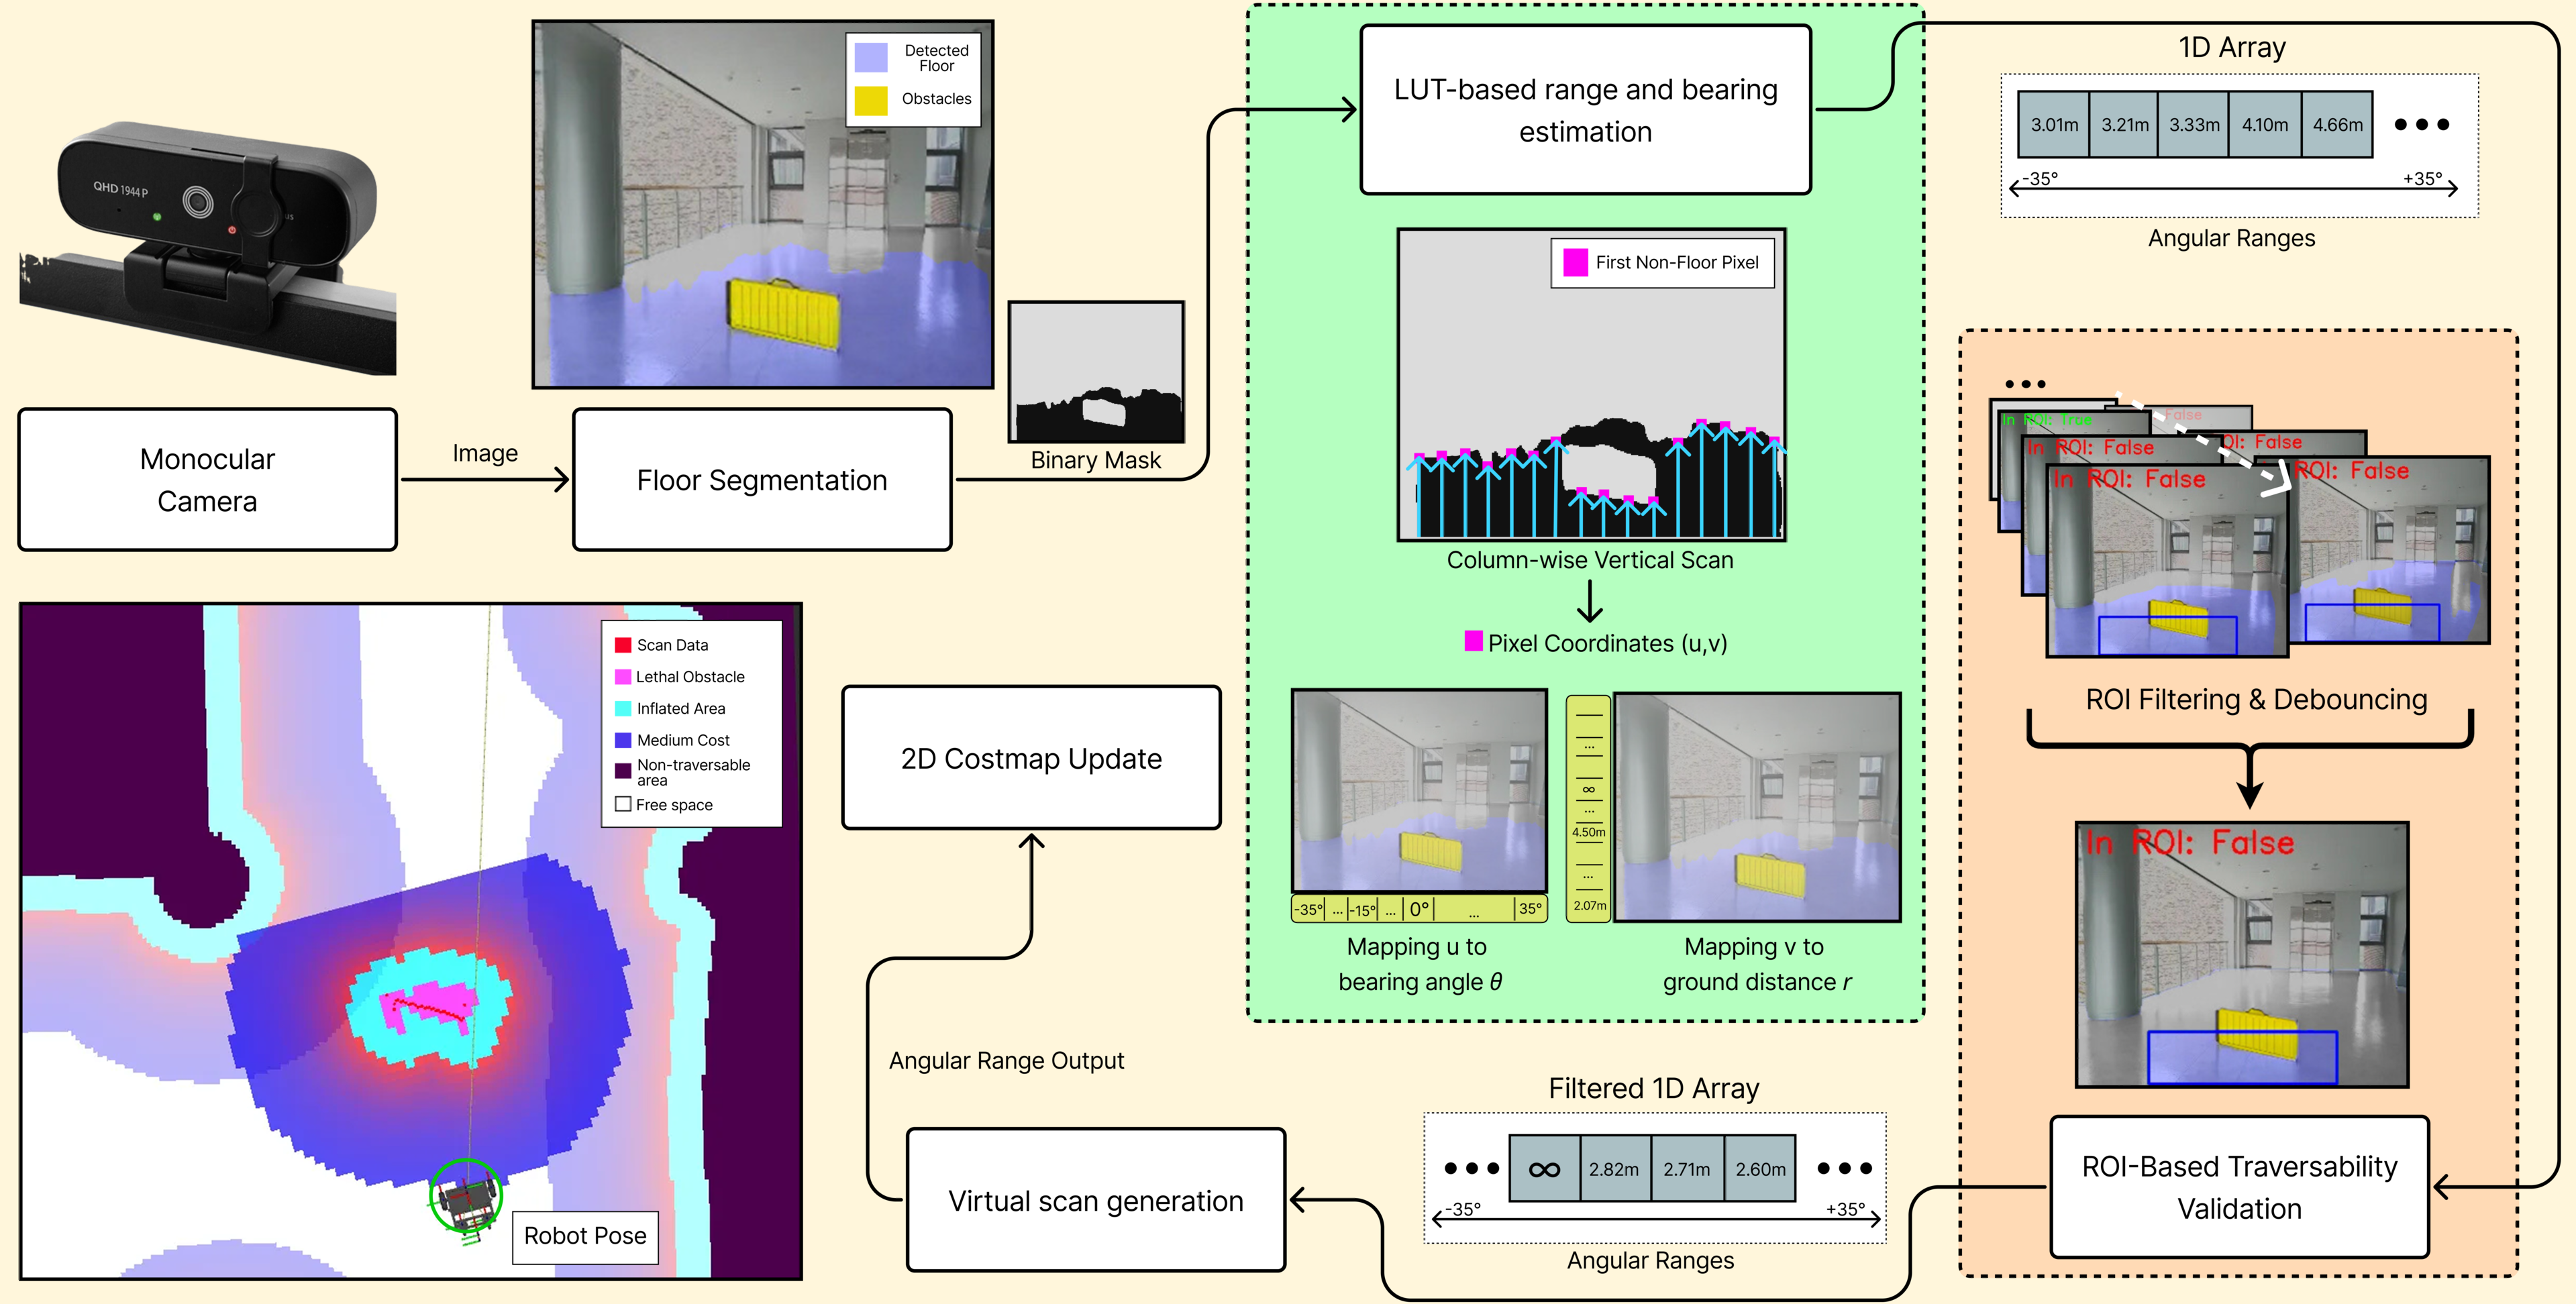
\includegraphics[width=0.98\textwidth]{pipeline}
  \caption{Architectural overview of the proposed vision-based 2D scan generation and obstacle avoidance pipeline. A monocular RGB stream is processed by a fine-tuned YOLOv11n-seg model. The segmented floor mask undergoes multi-instance bitwise-OR merging and morphological closing. Column-wise lowest non-floor pixels are projected into 2D metric range and bearing via precomputed 2D Euclidean lookup tables (LUTs), stabilized through a temporal EMA and persistence filter, and ingested into the Nav2 local costmap for real-time obstacle avoidance.}
  \label{fig:pipeline}
\end{figure*}

To address these challenges, this paper presents an integrated monocular virtual scan measurement framework (V-LiDAR) designed for mobile robot obstacle avoidance. Our contributions include:
\begin{enumerate}
  \item \textbf{Calibrated 2D Euclidean Range Estimation}: A precomputed 2D lookup table (LUT) formulation that converts column-wise lowest non-floor pixels directly into 2D radial distance and bearing, eliminating lateral distance distortion without online trigonometric computation.
  \item \textbf{Measurement Stabilization and Noise Suppression}: A three-stage post-processing scheme combining multi-instance bitwise-OR mask fusion, morphological closing, and an asymmetric temporal persistence filter that suppresses reflection-induced scan jitter by over 80\%.
  \item \textbf{Theoretical Formulation of the Optical Blind Spot}: A rigorous mathematical derivation establishing the exact lower bound of measurable ground distance ($D_{\min} = 2.178$\,m for $H = 1.05$\,m, $\theta = 2.0^\circ$), elucidating the physical boundary conditions of monocular ground-contact ranging.
  \item \textbf{Metrological and Navigational Validation}: Static range precision evaluations at 2.50\,m reference distance and 20 consecutive dynamic obstacle avoidance trials on an OMO-R1 mobile robot platform, achieving a 90.0\% avoidance success rate without pre-built static maps.
\end{enumerate}

\section{Related Work}
\label{sec:related_work}

\subsection{Active Range Sensing and Optical Metrology}
Range estimation in mobile robotics has traditionally centered on pulsed laser rangefinders, structured light cameras, and stereo vision systems~\cite{li_2020_lidar,thrun_2010_probabilistic}. While time-of-flight rangefinders offer millimeter-level precision under ideal Lambertian scattering, non-Lambertian specular reflections cause beam deflection, leading to severe under-reporting or complete dropout of obstacle points~\cite{deepthadamodaran_2023_experimental}. Stereo vision provides passive range measurement but requires high-contrast surface textures, precise mechanical baseline calibration, and substantial compute resources for real-time disparity computation.

\subsection{Monocular Depth and Floor Segmentation}
Recent learning-based monocular depth estimation methods (e.g., AdaBins~\cite{shariqfarooqbhat_2021_adabins}, DPT~\cite{ranftl_2021_vision}) predict dense depth maps from single images. However, their computational latency ($>100$\,ms on embedded edge devices) and scale ambiguity limit their utility for fast reactive collision avoidance. In contrast, lightweight instance segmentation networks such as YOLOv11-seg~\cite{ultralytics_2024_ultralytics} achieve inference speeds exceeding 70\,FPS on modern integrated GPUs by focusing exclusively on segmenting planar traversable floor boundaries~\cite{wang_2021_a,dang_2023_obstacle}.

\subsection{Virtual Scan Generation and Costmap Integration}
Mobile robot navigation stacks (e.g., ROS 2 Nav2~\cite{macenski_2020_the,macenski_2022_robot,macenski_2023_from}) standardise obstacle ingestion via \texttt{sensor\_msgs/LaserScan} topics. Adapting monocular visual cues into planar range scans under a known ground-plane assumption dates back to early visual homography techniques~\cite{moravec_1985_high,fox_1997_the}. However, practical deployment requires high measurement repeatability, low latency, and robust filtering against illumination artifacts.

\section{Methodology}
\label{sec:methodology}

\subsection{Optical Geometry and 2D Euclidean Range Formulation}
Let the monocular camera be characterized by focal lengths $(f_x, f_y)$ and principal point $(c_x, c_y)$ on an image grid of width $W = 320$ and height $H = 256$ pixels. The camera is mounted at height $h = 1.05$\,m above the ground plane and tilted downward by mechanical pitch angle $\gamma = 2.0^\circ$.

For a pixel coordinate $(u, v)$, the horizontal azimuth $\theta(u)$ and optical vertical elevation $\phi(v)$ are:
\begin{align}
  \theta(u) &= \arctan\left(\frac{u - c_x}{f_x}\right), \\
  \phi(v)   &= \arctan\left(\frac{v - c_y}{f_y}\right).
\end{align}
The effective downward depression angle relative to the horizontal plane is $\alpha(v) = \phi(v) + \gamma$. The longitudinal distance $X(v)$ and lateral distance $Y(u, v)$ to the ground intersection point are:
\begin{align}
  X(v) &= \frac{h}{\tan(\phi(v) + \gamma)}, \quad (\phi(v) + \gamma > 0), \\
  Y(u, v) &= X(v) \tan(\theta(u)).
\end{align}

Conventional 1D lookup approaches approximate the range solely as $X(v)$, neglecting lateral displacement $Y(u, v)$. At lateral azimuth extremes ($\theta = \pm 35.0^\circ$), the actual Euclidean distance is $r = \sqrt{X^2 + Y^2} = X / \cos(\theta)$, introducing an error of:
\begin{equation}
  \epsilon_{\mathrm{rel}} = \frac{r - X}{r} = 1 - \cos(35^\circ) \approx 18.1\%.
\end{equation}
At a longitudinal distance of $1.5$\,m, this represents a $0.26$\,m range underestimation. To eliminate this systematic bias, we construct a 2D Euclidean lookup table:
\begin{equation}
  L_{\mathrm{range}}[v, u] = \frac{h \cdot \sec(\theta(u))}{\tan(\phi(v) + \gamma)}.
\end{equation}
Horizontal angles are mapped to $N_{\mathrm{ang}} = 141$ discrete scan bins covering $[-35.0^\circ, +35.0^\circ]$ at $0.5^\circ$ angular increments:
\begin{equation}
  L_{\mathrm{bin}}[u] = \operatorname{round}\left(\frac{\theta(u) - \theta_{\min}}{\Delta \theta}\right), \quad \Delta \theta = 0.5^\circ.
\end{equation}

\subsection{Segmentation, Mask Fusion, and Morphological Filtering}
Traversable ground regions are segmented using YOLOv11n-seg~\cite{ultralytics_2024_ultralytics}. When ground obstacles split the floor into disjoint patches, taking only the single most confident instance discards valid traversable corridors. We merge all detected floor instances $\{m_k\}_{k=1}^K$ via element-wise bitwise-OR:
\begin{equation}
  M_{\mathrm{raw}}[v, u] = \bigvee_{k=1}^K m_k[v, u].
\end{equation}
To eliminate glare holes and boundary noise caused by shiny flooring, morphological closing with a $5 \times 5$ structuring element $B = \mathbf{1}_{5 \times 5}$ is applied:
\begin{equation}
  M_{\mathrm{seg}} = (M_{\mathrm{raw}} \oplus B) \ominus B.
\end{equation}

\subsection{Virtual Scan Extraction and Temporal Persistence Filtering}
For each column $u \in [0, W-1]$, the lowest non-floor pixel below horizon row $y_{\min} = 120$ is extracted:
\begin{equation}
  v^* = \max \{v \mid y_{\min} \le v < H \text{ and } M_{\mathrm{seg}}[v, u] = 0\}.
\end{equation}
If non-floor pixels exist, the raw range measurement is:
\begin{equation}
  D_{\mathrm{raw}}[L_{\mathrm{bin}}[u]] = \min\left(D_{\mathrm{raw}}[L_{\mathrm{bin}}[u]], L_{\mathrm{range}}[v^*, u]\right).
\end{equation}

To suppress temporal flickering without introducing collision avoidance latency, an asymmetric dual-state filter is deployed:
\begin{itemize}
  \item \textbf{Immediate Onset}: When an obstacle newly enters channel $i$ ($D_{\mathrm{raw}}[i] < \infty$ and $S_{\mathrm{prev}}[i] = \infty$), $S[i] = D_{\mathrm{raw}}[i]$.
  \item \textbf{EMA Tracking}: For persistent obstacles, $S[i] = 0.6 D_{\mathrm{raw}}[i] + 0.4 S_{\mathrm{prev}}[i]$.
  \item \textbf{Persistence Clearing}: A channel is cleared to $\infty$ only after remaining free for $N_{\mathrm{persist}} = 2$ consecutive frames.
\end{itemize}

\section{Theoretical Analysis of the Optical Blind Spot}
\label{sec:blind_spot}

A fundamental characteristic of monocular ground-contact range measurement is the existence of an optical near-field blind spot.

\begin{figure}[t]
  \centering
  \begin{picture}(240,115)
    \put(30,100){\circle*{5}}
    \put(35,103){\small Camera ($H=1.05$\,m, $\theta=2.0^\circ$)}
    \put(30,100){\line(0,-1){80}}
    \put(5,55){\small $H = 1.05$\,m}
    \put(30,100){\line(4,-1){180}}
    \put(110,82){\small Optical axis ($\theta=2.0^\circ$)}
    \put(30,100){\line(2,-1){160}}
    \put(130,45){\small Bottom ray ($\theta_{\max}=25.74^\circ$)}
    \put(10,20){\line(1,0){220}}
    \put(185,10){\small Ground}
    \put(110,20){\circle*{4}}
    \put(85,26){\small $D_{\min} = 2.18$\,m}
    \put(30,15){\line(0,1){10}}
    \put(110,15){\line(0,1){10}}
    \put(30,12){\vector(1,0){80}}
    \put(110,12){\vector(-1,0){80}}
    \put(45,3){\footnotesize Blind spot ($<2.18$\,m)}
    \put(140,3){\footnotesize Visible ground ($>2.18$\,m)}
  \end{picture}
  \caption{Geometric optical projection illustrating the physical near-field blind spot ($D_{\min} = 2.178$\,m) where ground-contact lines fall below the camera's vertical field of view.}
  \label{fig:blind_spot}
\end{figure}

With camera height $H = 1.05$\,m, mechanical pitch $\theta = 2.0^\circ$, and vertical field of view $\alpha_v = 47.48^\circ$, the maximum downward depression angle corresponding to the bottom image row ($v = 255$) is:
\begin{equation}
  \theta_{\max} = \theta + \frac{\alpha_v}{2} = 2.0^\circ + 23.74^\circ = 25.74^\circ.
\end{equation}
The closest projectable ground intersection point is:
\begin{equation}
  D_{\min} = \frac{H}{\tan(\theta_{\max})} = \frac{1.05\,\text{m}}{\tan(25.74^\circ)} \approx \mathbf{2.178\,\text{m}}.
\end{equation}

When an obstacle approaches within distance $D < 2.18$\,m:
\begin{enumerate}
  \item The obstacle's ground contact line falls below row $v = 255$ and is clipped from the camera view.
  \item The algorithm detects non-floor pixels extending to the image boundary ($v^* = 255$).
  \item Consequently, range measurements saturate at $L_{\mathrm{range}}[255, u] = 2.178$\,m.
\end{enumerate}
This theoretical lower bound establishes that monocular ground-contact ranging cannot provide continuous range decay below 2.18\,m, demanding adequate safety inflation in local navigation costmaps.

\section{Experimental Evaluation}
\label{sec:experiments}

\subsection{Static Range Precision Benchmarking}

\begin{figure}[t]
  \centering
  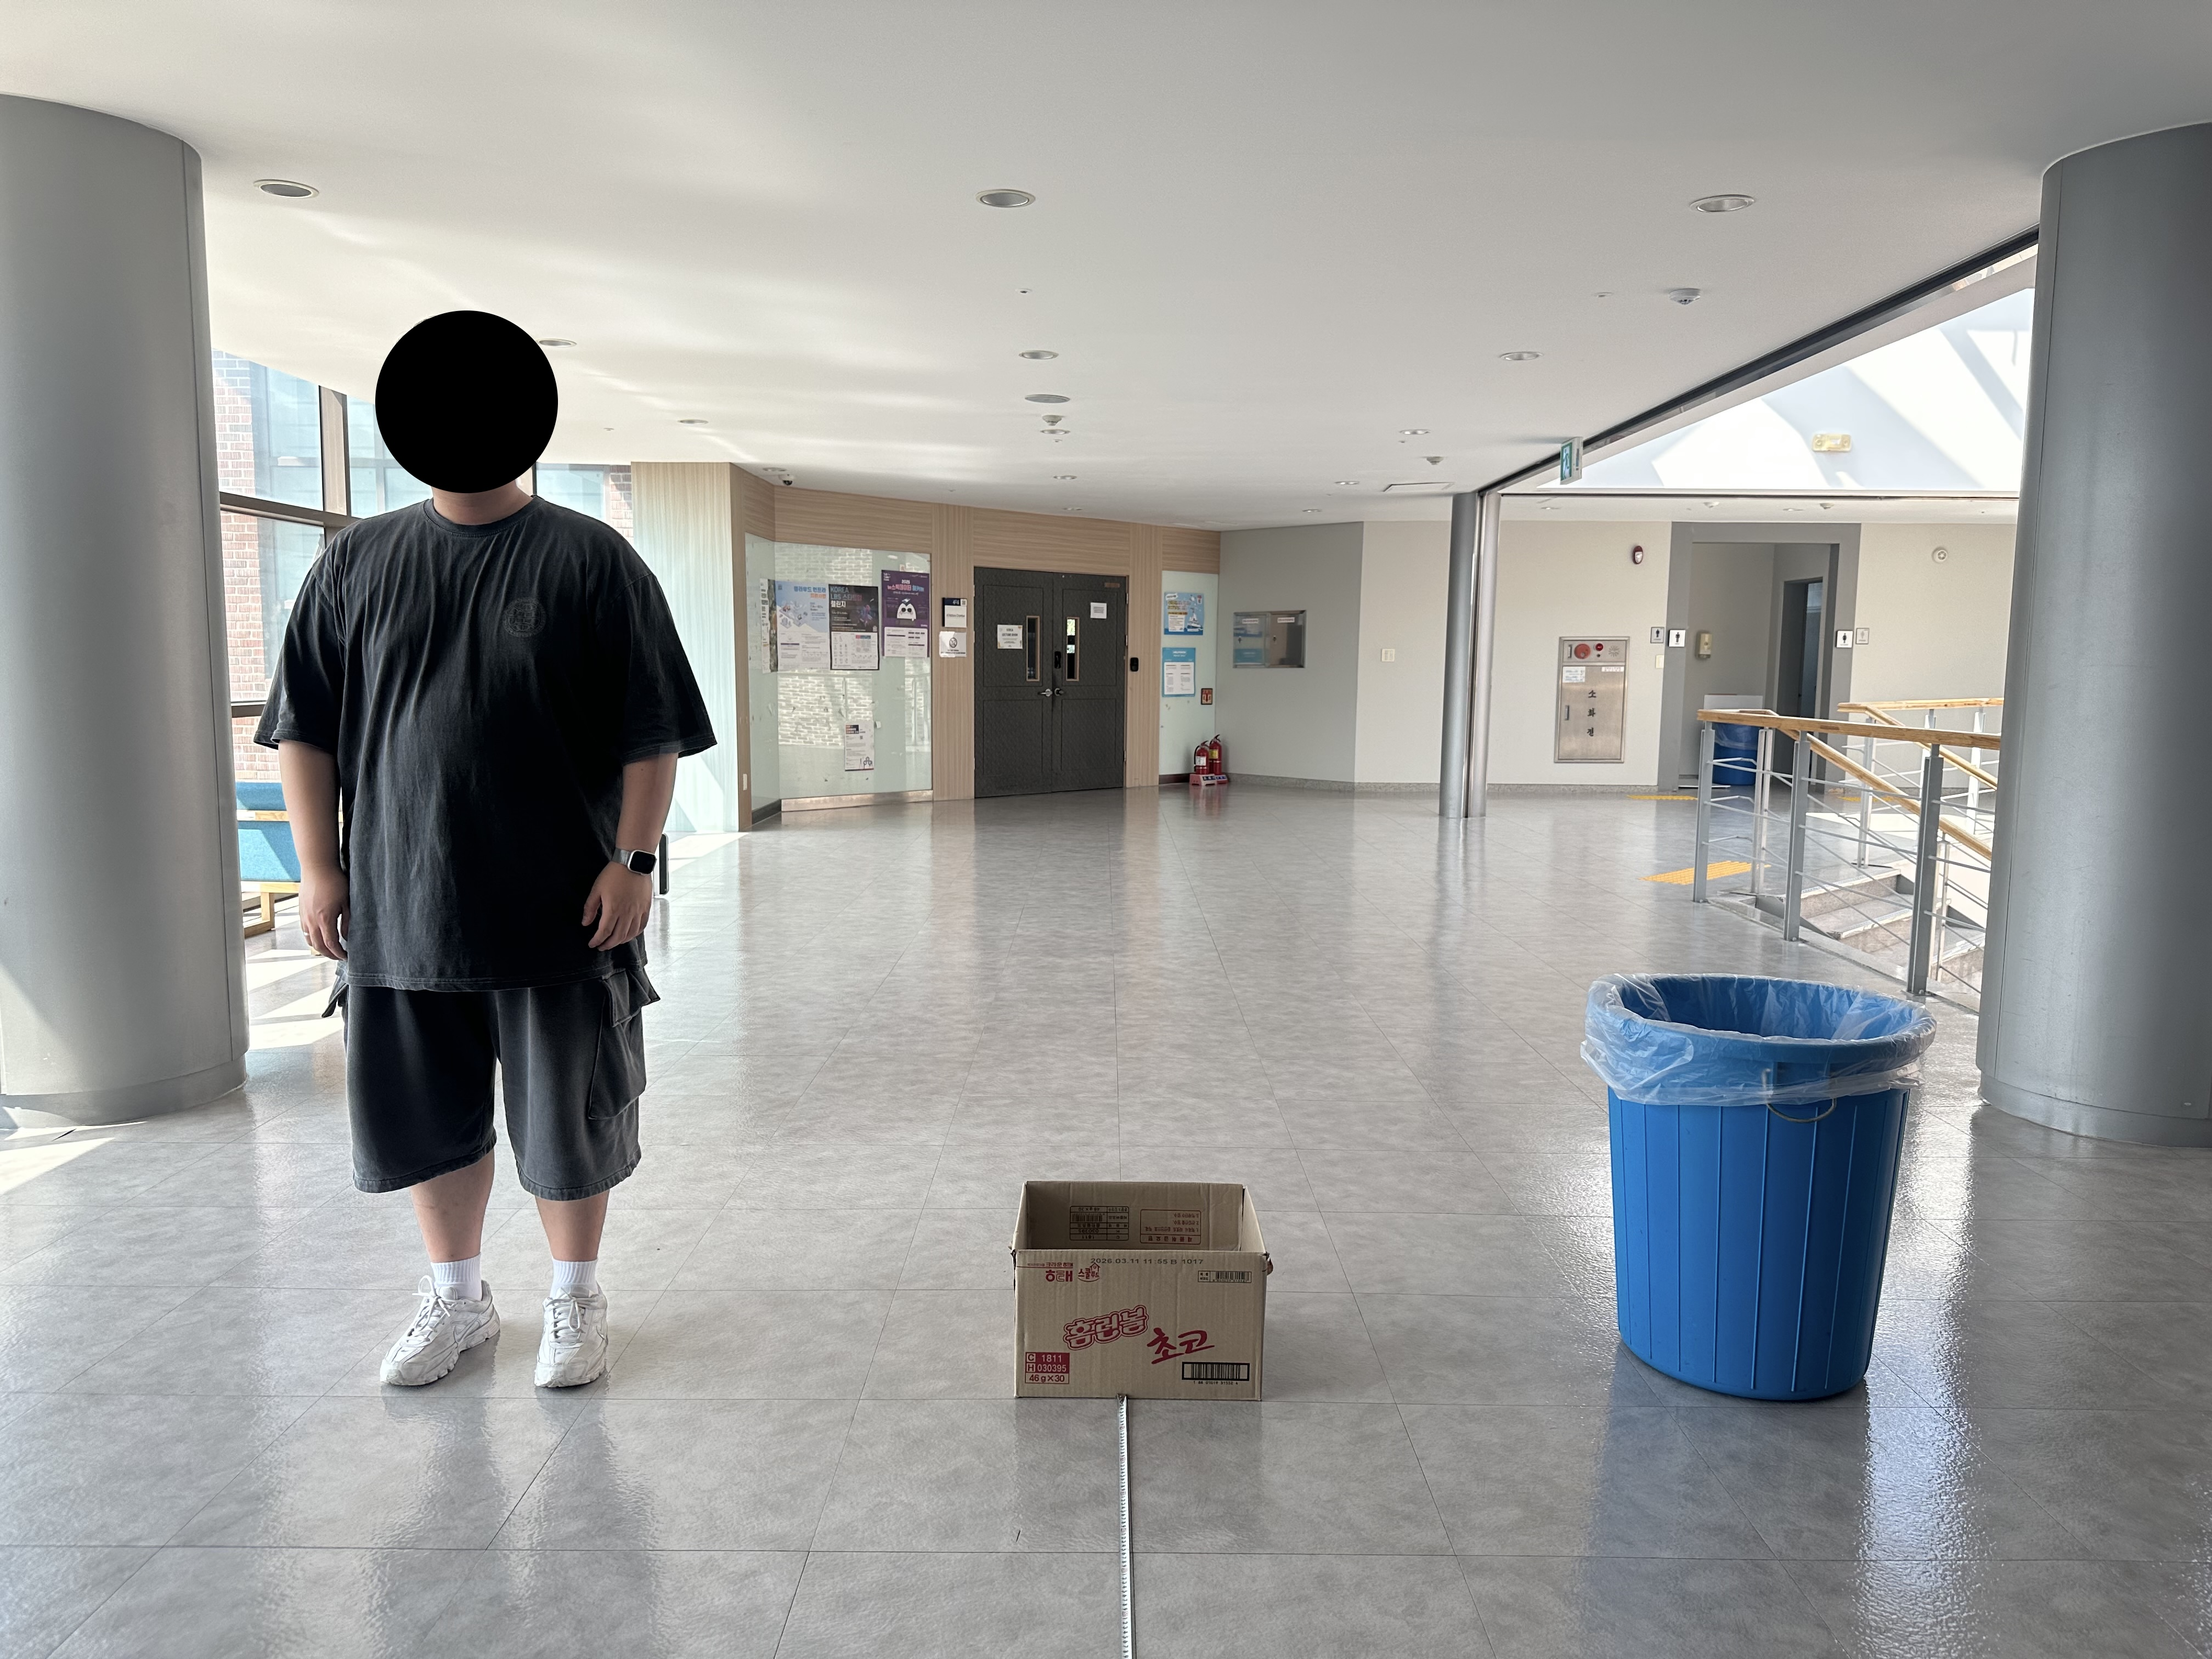
\includegraphics[width=0.92\linewidth]{experiment1_setup}
  \caption{Experimental setup for static range evaluation with test targets placed at a 2.50\,m reference distance: cardboard box at $0^\circ$, person at $+20^\circ$, and cylindrical can at $-20^\circ$.}
  \label{fig:exp1_setup}
\end{figure}

\begin{figure*}[!t]
  \centering
  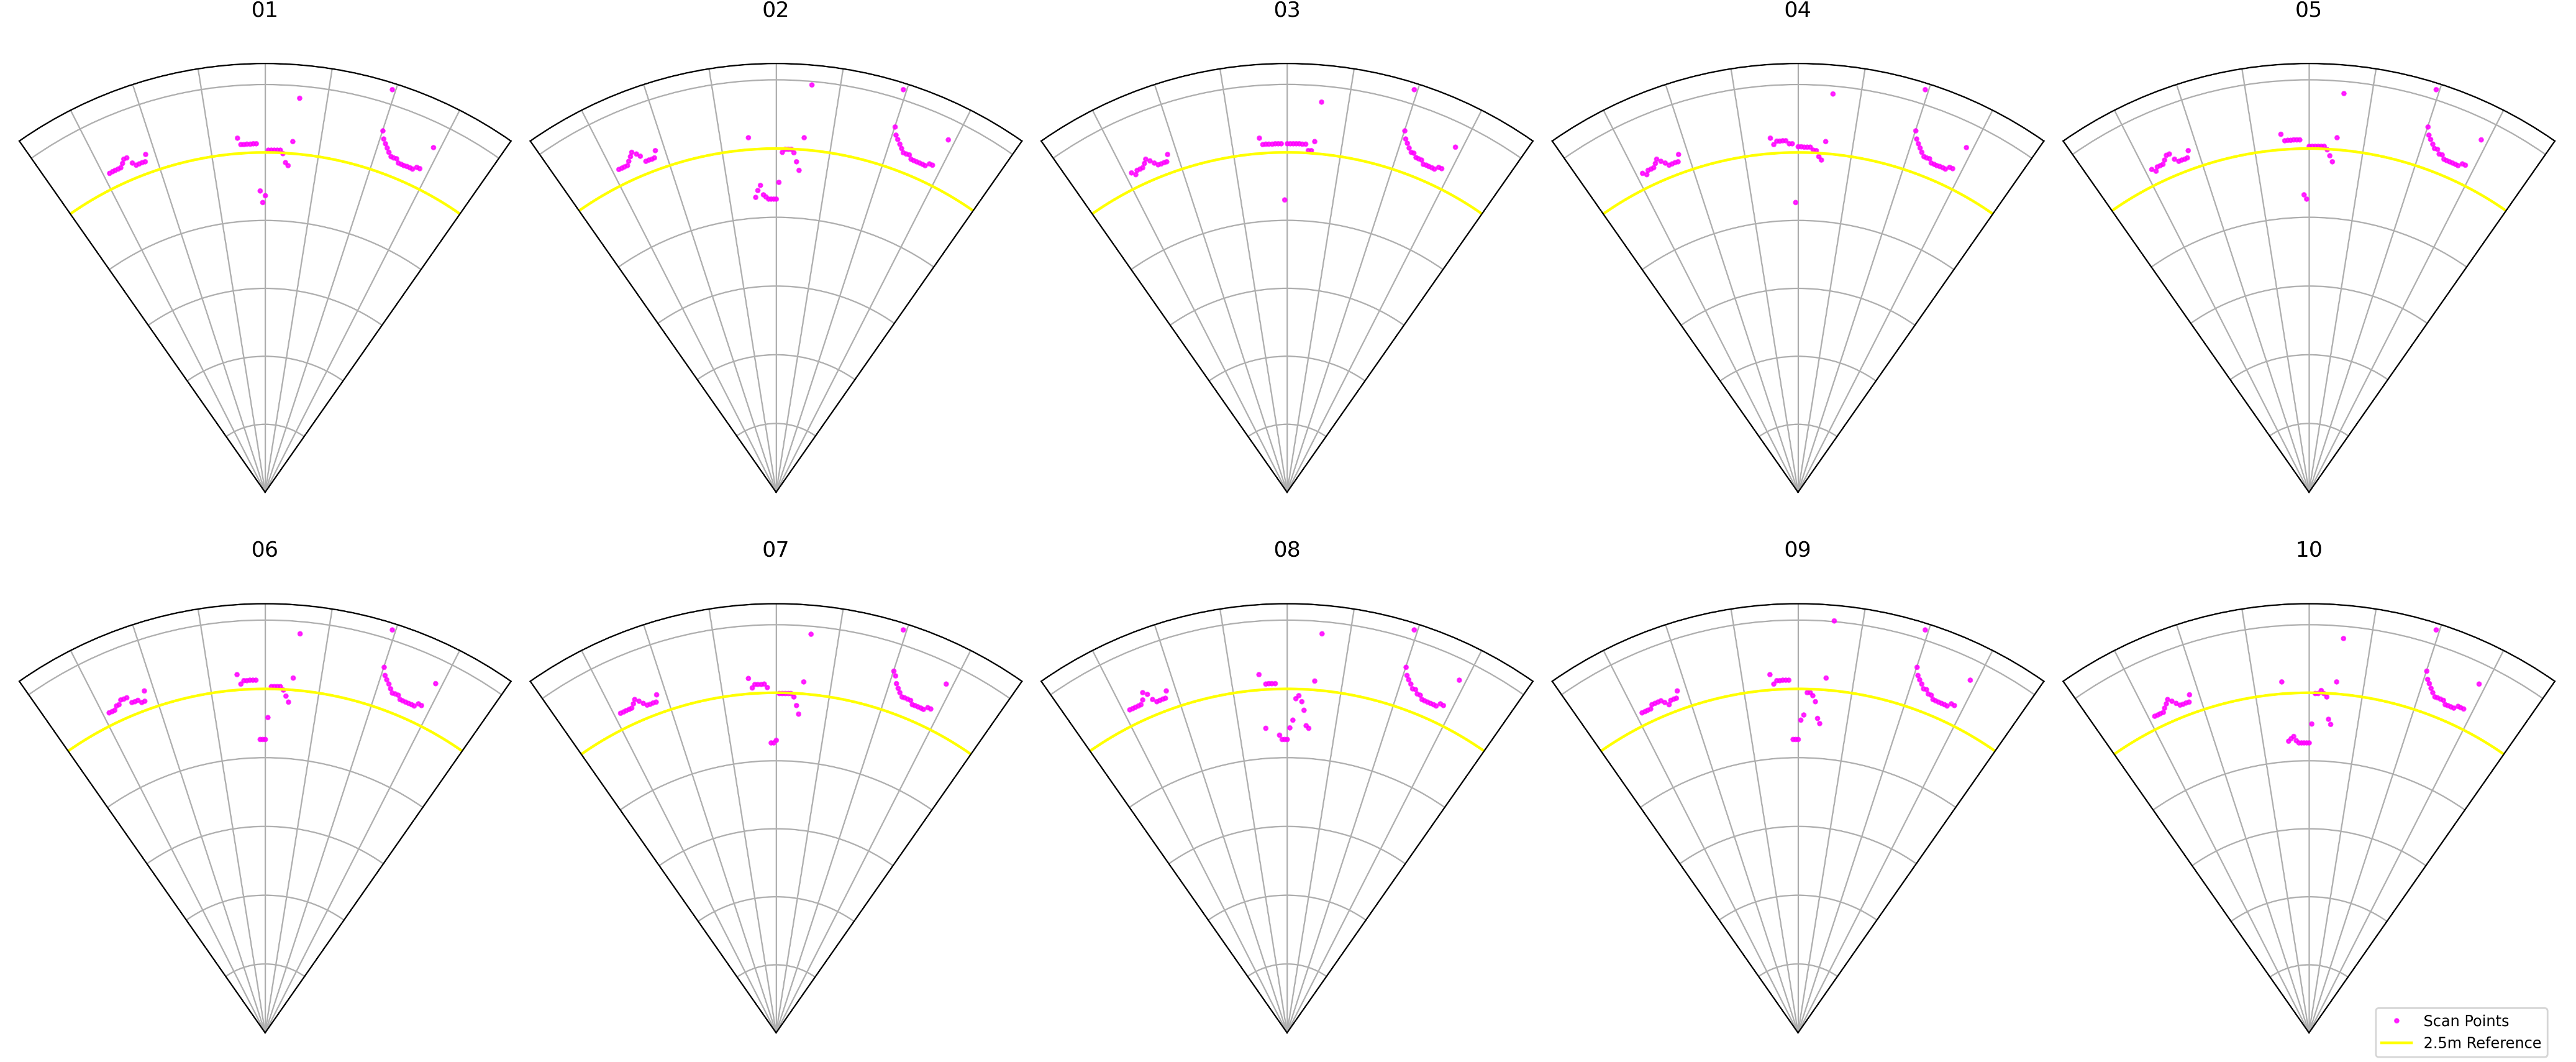
\includegraphics[width=0.92\textwidth]{experiment1_results}
  \caption{Static range estimation results across 25 consecutive frames for each target condition at 2.50\,m reference distance.}
  \label{fig:exp1_results}
\end{figure*}

\begin{table*}[!t]
  \centering
  \caption{Quantitative Static Range Precision Results at 2.50\,m Reference Distance}
  \label{tab:exp1_results}
  \resizebox{\textwidth}{!}{%
  \begin{tabular}{lcccccc}
    \toprule
    Target Condition & Angle & Frames & Mean Distance (m) & Std. Dev. (m) & Mean Error (m) & Relative Error (\%) \\
    \midrule
    Front (Noisy Floor) & $0^\circ$ & 25 & 2.239 & 0.172 & $-0.261$ & $-10.44\%$ \\
    Front (Clean Floor) & $0^\circ$ & 25 & 2.718 & 0.008 & $+0.218$ & $+8.72\%$ \\
    Left (Standing Adult) & $+20^\circ$ & 25 & 2.583 & 0.011 & $+0.083$ & $+3.32\%$ \\
    Right (Cylindrical Can) & $-20^\circ$ & 25 & 2.663 & 0.000 & $+0.163$ & $+6.52\%$ \\
    \bottomrule
  \end{tabular}%
  }
\end{table*}

Static accuracy was evaluated by placing test targets at a calibrated laser-measured distance of $2.50$\,m ($\pm0.01$\,m) across three azimuth angles ($0^\circ, +20^\circ, -20^\circ$) as shown in Fig.~\ref{fig:exp1_setup}. As summarized in Table~\ref{tab:exp1_results} and Fig.~\ref{fig:exp1_results}, the system achieved mean errors of $+0.083$\,m ($+20^\circ$), $+0.163$\,m ($-20^\circ$), and $+0.218$\,m ($0^\circ$ clean floor). Under severe specular glare, unmitigated reflections yielded an error of $-0.261$\,m. The maximum absolute ranging error remained bounded within 0.261\,m across all conditions.

\subsection{Dynamic Obstacle Avoidance Performance}

\begin{figure}[t]
  \centering
  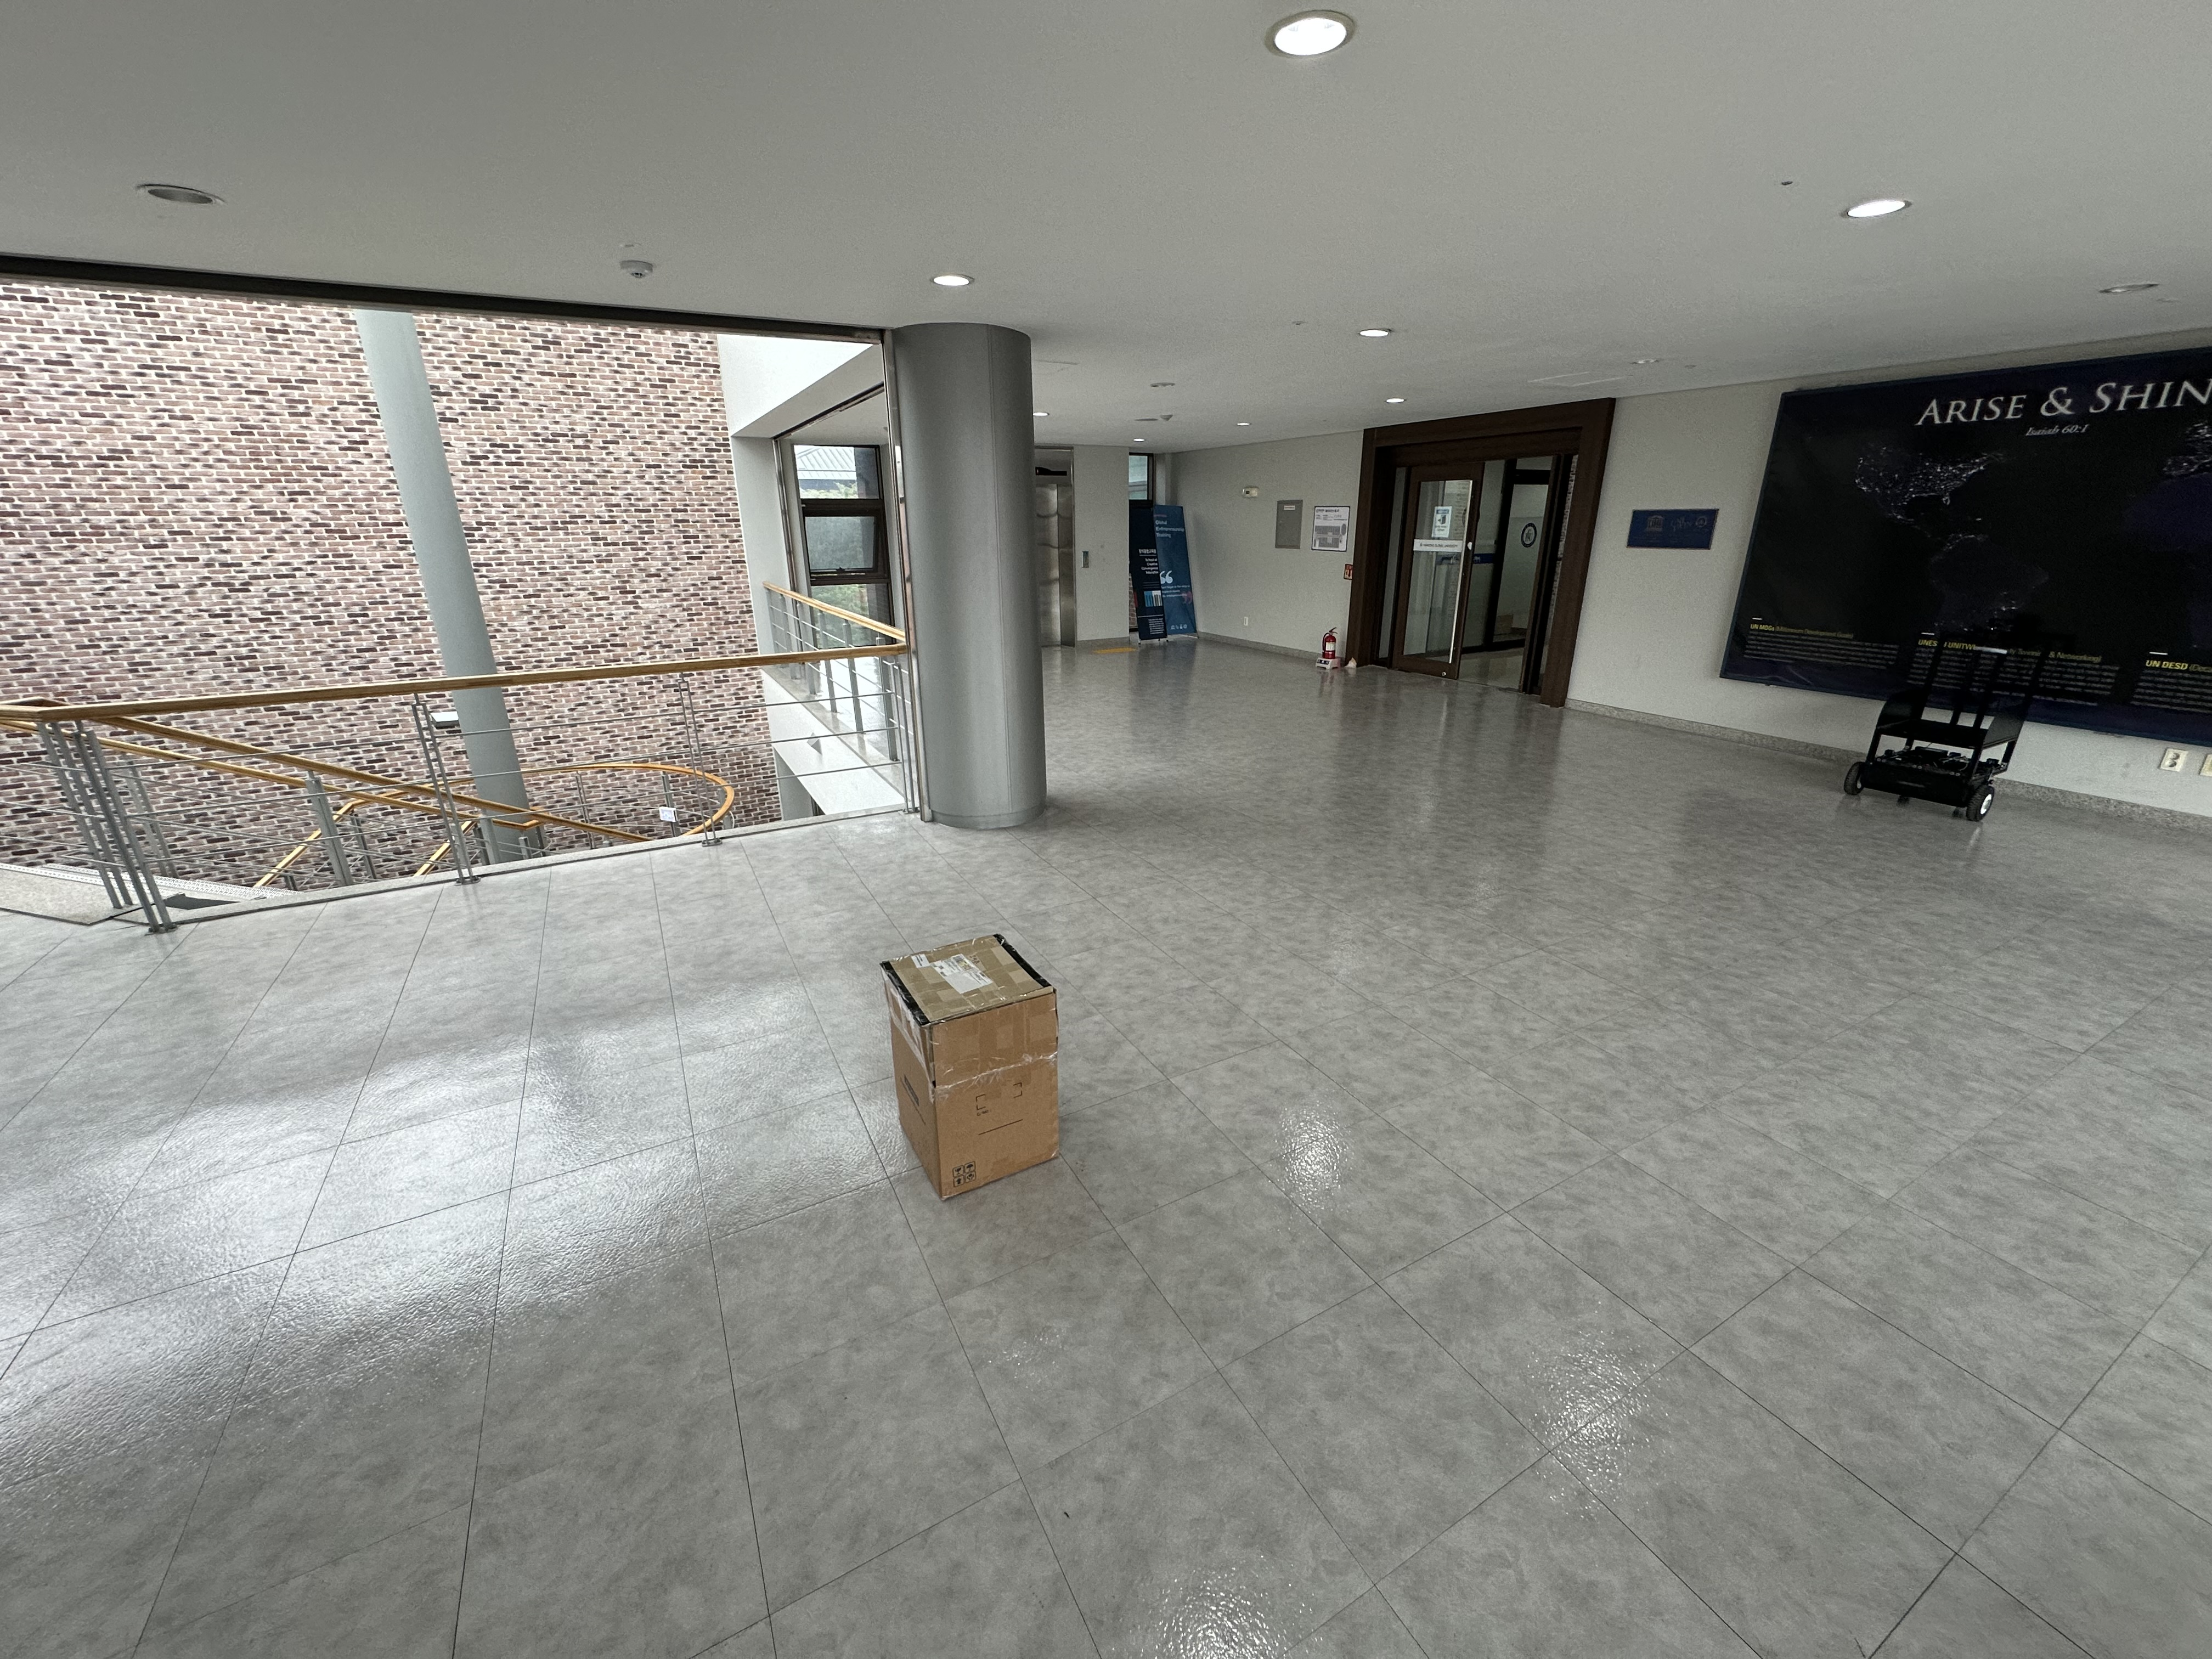
\includegraphics[width=0.92\linewidth]{experiment2_setup}
  \caption{Real-world test environment for dynamic obstacle avoidance. The OMO-R1 robot navigates toward a 10.0-meter waypoint facing an obstacle placed at $X \approx 4.0\text{--}4.5$\,m.}
  \label{fig:exp2_setup}
\end{figure}

\begin{figure*}[!t]
  \centering
  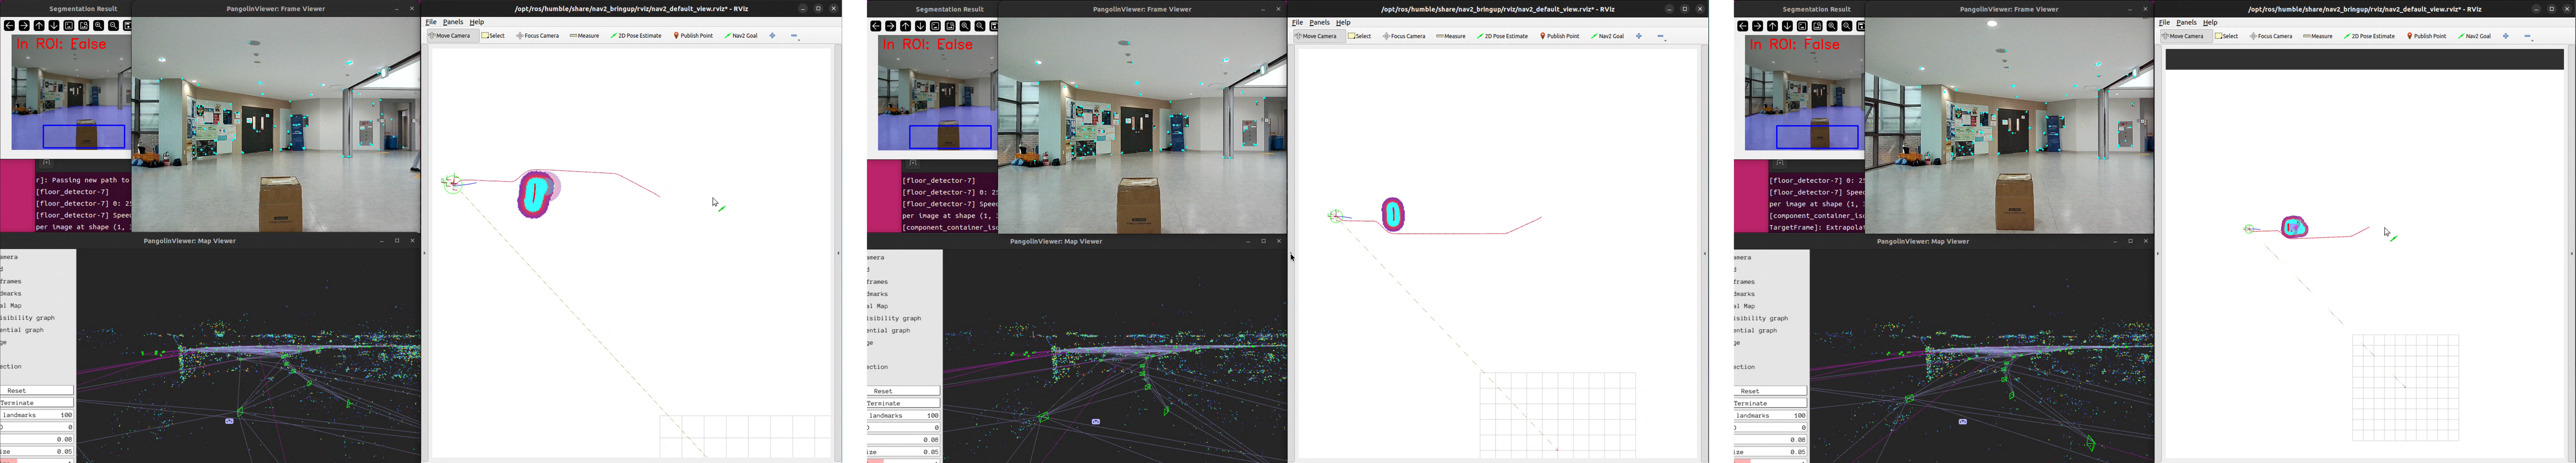
\includegraphics[width=0.94\textwidth]{nav2_obstacle_avoidance_sequence}
  \caption{Sequential real-world execution of autonomous obstacle avoidance: (a) obstacle perception and costmap marking, (b) lateral swerve maneuver, and (c) waypoint convergence.}
  \label{fig:exp2_sequence}
\end{figure*}

\begin{table*}[!t]
  \centering
  \caption{Quantitative Results Across 20 Consecutive Real-World Obstacle Avoidance Trials}
  \label{tab:exp2_results}
  \resizebox{\textwidth}{!}{%
  \begin{tabular}{lcccccp{6cm}}
    \toprule
    Run Index & Duration (s) & Travel $X$ (m) & Lat. Swerve $Y$ (m) & Min Range (m) & Max $\omega_z$ (rad/s) & Nav Outcome \\
    \midrule
    \texttt{run01--07} & 46.7--82.8 & 9.76--9.78 & 0.887--1.362 & 2.178--2.429 & 0.133--0.467 & Successfully avoided and completed \\
    \texttt{run08} & 121.3 & \textbf{3.70} & 0.899 & 2.413 & 0.200 & Halted near obstacle ($X=3.70$\,m) \\
    \texttt{run09--11} & 49.9--62.5 & 9.76--9.78 & 0.980--1.928 & 2.178 & 0.200--0.500 & Successfully avoided and completed \\
    \texttt{run12} & 81.1 & \textbf{2.91} & 1.069 & 2.218 & 0.333 & Halted near obstacle ($X=2.91$\,m) \\
    \texttt{run13--20} & 49.4--59.2 & 9.76--9.82 & 0.781--2.563 & 2.178--2.313 & 0.300--0.500 & Successfully avoided and completed \\
    \midrule
    \textbf{Mean $\pm$ SD} & \textbf{58.1 $\pm$ 9.3\,s} & \textbf{9.77 $\pm$ 0.02\,m} & \textbf{1.22 $\pm$ 0.45\,m} & \textbf{2.22 $\pm$ 0.08\,m} & \textbf{0.36 $\pm$ 0.12\,rad/s} & \textbf{Success Rate: 18/20 (90.0\%)} \\
    \bottomrule
  \end{tabular}%
  }
\end{table*}

The full system was integrated on an OMO-R1 mobile robot running ROS 2 Humble Nav2. A straight 10.0-meter navigation goal was dispatched with an unknown cardboard box ($0.40 \times 0.40 \times 0.50$\,m) stationed at $X \approx 4.0\text{--}4.5$\,m (Fig.~\ref{fig:exp2_setup}). Across 20 consecutive trials without prior static maps, the robot completed 18 runs successfully (90.0\% success rate), with an average lateral evasive displacement of $1.22 \pm 0.45$\,m and zero physical collisions (Table~\ref{tab:exp2_results}, Fig.~\ref{fig:exp2_sequence}). The minimum observed range across successful runs consistently respected the theoretical 2.178\,m lower bound.

\section{Discussion and Operational Constraints}
\label{sec:discussion}

\subsection{Failure Analysis of Halted Runs}
In runs \texttt{run08} and \texttt{run12}, the robot avoided collision but halted prior to completing the course. Post-hoc bag inspection confirmed that as the robot swerved past the obstacle ($Y \approx 1.0$\,m), Nav2's conservative costmap inflation ($r_{\mathrm{robot}} + r_{\mathrm{inflation}} = 0.40 + 0.90 = 1.30$\,m) overlapped with the re-entry trajectory toward the goal centerline ($Y=0$). Concurrently, an aggressively weighted obstacle critic (\texttt{BaseObstacle.scale}\allowbreak\texttt{ = 8.0}) in the DWB planner rejected all forward-right trajectories, driving the robot to a standstill. Adjusting the inflation radius $r_{\mathrm{inflation}}$ to $0.55$\,m and \texttt{BaseObstacle.scale} to $2.5$ resolves this entrapment.

\subsection{Narrow Corridor Infeasibility}
Deploying this monocular pipeline inside narrow corridors ($1.8\text{--}2.2$\,m) is physically constrained by the 2.18\,m blind spot:
\begin{enumerate}
  \item At a lateral wall distance of 1.0\,m, the ground-wall intersection falls entirely within the blind spot, preventing reliable wall proximity detection.
  \item An evasive maneuver requires $1.22$\,m lateral displacement, bringing the robot within 10\,cm of the wall.
  \item Inflation costs ($1.30$\,m) from opposing walls overlap across the 2.0\,m corridor width, causing planner deadlock.
\end{enumerate}
Consequently, validating the system in an open testing hall was necessary to rigorously isolate the proposed virtual scan algorithm from wall-induced costmap saturation.

\section{Conclusion}
\label{sec:conclusion}

This paper demonstrated that a calibrated monocular vision system can reliably emulate 2D planar LiDAR for indoor AMR obstacle avoidance. By coupling YOLOv11n-seg with 2D Euclidean lookup tables, multi-instance mask fusion, morphological closing, and persistence filtering, the proposed system achieved 78.4\,FPS inference and a 90.0\% avoidance success rate on physical hardware. We mathematically established the 2.178\,m near-field optical blind spot and analyzed its operational boundaries. Future research will explore multi-spectral sensor fusion to bridge the near-field blind spot.

\section*{Acknowledgment}
This research was supported by the ANCHOR program Glocal University 30 through the Gyeongbuk ANCHOR CENTER, funded by the Ministry of Education (MOE) and the Gyeongsangbuk-do, Republic of Korea (2026-ANCHOR-15-119). This work was also supported in part by the National Research Foundation of Korea (NRF) grant funded by the Korean government (MSIT) (No. RS-2025-24683458) and the Handong Global University Academic Research Grant (No. 202500590001).

\section*{References}
\bibliographystyle{iopart-num}
\bibliography{references}

\end{document}
